\section{Scaling laws for repeated data}
\label{sec:method}

\para{Limitations of the effective-data approach.} We begin by examining where the \citet{muennighoff2023scaling} formulation breaks down. Figure~\ref{fig:muennighoff_residuals} plots predicted vs.\ observed validation loss under the Chinchilla baseline and the $\widehat{D}(U_D, R_D), \widehat{N}(U_N, R_N)$ form across four model sizes. Two patterns emerge: first, the gap between predicted and observed loss grows with the number of repetitions, indicating that the effective-data forms systematically underpredict loss at high epoch counts. Second, the gap increases with model capacity relative to unique data, confirming an interaction between model size and repetition that the exponential saturation in $\widehat{D}(U_D, R_D)$ and $\widehat{N}(U_N, R_N)$ cannot capture.

\begin{figure}[t]
    \centering
    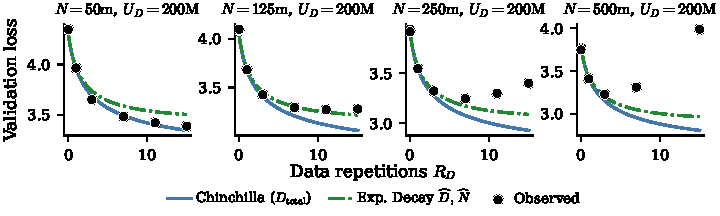
\includegraphics[width=\textwidth]{figures/muennighoff_residuals.pdf}
    \caption{\textbf{Existing scaling laws fail to model overfitting.} Predicted vs.\ observed validation loss under the Chinchilla baseline (treating repeated tokens as unique) and the \citet{muennighoff2023scaling} $\widehat{D}(U_D, R_D), \widehat{N}(U_N, R_N)$ formulation across four model sizes at $U_D = 200$M. Both formulations fail to capture the loss increase at high repetition counts, systematically underpredicting loss as repetitions grow.}
    \label{fig:muennighoff_residuals}
    \vspace{-1em}
\end{figure}

\para{An additive overfitting penalty.} To identify the right functional form, we fit the Chinchilla law (Equation~\ref{eq:chinchilla}) to single-epoch runs, obtaining parameters $(E, A, B, \alpha, \beta)$, and use this fit to predict multi-epoch loss by treating repeated tokens as if they were fresh data $D = U_D \cdot (1 + R_D)$. The residual between the observed loss and this prediction isolates the additional cost attributable to repetition.
When we plot this residual for a fixed model size $N$ and unique data budget $U_D$, varying only the number of repetitions $R_D$, a power-law relationship emerges (Figure~\ref{fig:residual_power}). A shared power-law fit $P_i \cdot R_D^\delta$ across all (model, budget) configurations, with $\delta$ tied and $P_i$ free per cell, finds the repetition damage is \emph{superlinear}. Each additional epoch of repetition inflicts more damage than the last.

\begin{figure}[t]
    \centering
    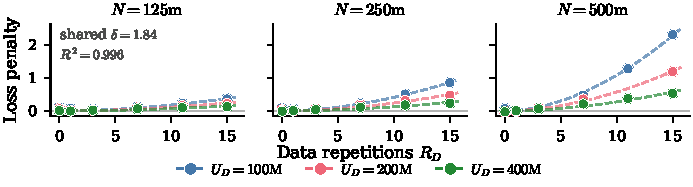
\includegraphics[width=\textwidth]{figures/residual_power.pdf}
    \caption{\textbf{The cost of repeating data grows superlinearly.} Residual between observed loss and the Chinchilla prediction (treating all repeated tokens as unique data) as a function of repetition count $R_D$, shown for three model sizes and three unique data budgets $U_D$. Dashed lines show power-law fits with a shared exponent $\delta$ across all configurations; the fitted $\delta > 1.0$ indicates superlinear repetition damage. Slopes are steeper for larger models and smaller unique data budgets.}
    \label{fig:residual_power}
    \vspace{-1em}
\end{figure}

\para{A complexity ladder of penalty forms.} Examining how the per-cell coefficient $P_i$ varies across configurations reveals its structure: larger models and smaller unique data budgets incur steeper penalties. This motivates a family of additive penalty forms of increasing complexity, which we present as a Pareto frontier trading off number of free parameters against fit quality.
The simplest form uses a single free parameter $P$ and the dimensionless ratio $N / U_D$:
\begin{equation}
    L(N, U_D, R_D) = E + \frac{A}{N^\alpha} + \frac{B}{\left(U_D \cdot (1 + R_D)\right)^\beta} + P \cdot R_D \cdot \frac{N}{U_D}.
    \label{eq:one_param}
\end{equation}
This linear-in-$R_D$ form already substantially outperforms the \citet{muennighoff2023scaling} formulations (Section~\ref{sec:validation}).
Adding a second free parameter, the exponent $\kappa$ on the capacity ratio, allows the penalty to scale nonlinearly with model size relative to data:
\begin{equation}
    L(N, U_D, R_D) = E + \frac{A}{N^\alpha} + \frac{B}{\left(U_D \cdot (1 + R_D)\right)^\beta} + P \cdot R_D \cdot \left(\frac{N}{U_D}\right)^\kappa.
    \label{eq:two_param}
\end{equation}
Across configurations, $\kappa > 1$, indicating that the overfitting penalty grows superlinearly with the ratio of model capacity to unique data.
The full four-parameter form adds a superlinear exponent $\delta$ on the repetition count and decouples the data-budget exponent $\gamma$ from the model-size exponent $\kappa$:
\begin{equation}
    L(N, U_D, R_D) = E + \frac{A}{N^\alpha} + \frac{B}{\left(U_D \cdot (1 + R_D)\right)^\beta} + P \cdot R_D^\delta \cdot \left(\frac{N}{U_D^\gamma}\right)^\kappa.
    \label{eq:four_param}
\end{equation}
% We observed that no three-parameter form lies on the Pareto frontier: $\kappa$ and $\gamma$ co-vary tightly and adding only one yields marginal improvement over the two-parameter form.

At $R_D = 0$ (single epoch), all three forms reduce exactly to the Chinchilla law. The key conceptual difference from the effective-data approach is that repeated tokens play a dual role: they continue to reduce the data-sufficiency term (they are not wasted) while simultaneously incurring a growing overfitting cost. 
% The \citet{muennighoff2023scaling} formulation collapses both effects into a single saturating quantity $\widehat{D}(U_D, R_D)$, treating repeated tokens as progressively less useful rather than as useful but costly. Our formulation also captures the interaction between model size, data budget, and overfitting through the penalty's capacity term, rather than through effective parameters that break the equivalence with the Chinchilla equation.
